\section{Thesis environment}
\label{sec:thesis_env}

\subsection{\acs*{plat} project}
\label{subsec:platinum}
This thesis is founded by the French \Ac{anr} institute and is part of the \href{http://platinum.projets.litislab.fr/}{\ac{plat}} project (ANR-15-CE23-0010). \Ac{plat} is a long-term mapping project composed of three parts: multi-source mapping, online navigation and map update. The first part is a offline map-building from multi-modal data sources that produces a high resolution textured mesh with photometric, geometric and semantic information. Then, this map is used as a reference for a online visual navigation module. During the navigation, an agent sends visual feedback to the server in order to update the map if changes are detected between the reference map and the current observation. The subject of this thesis focuses on the initial localization of the agent over the entire map before the start of the navigation.

\subsection{The localization task}
\paragraph{Summary of the map.}
The online localization task within the \ac{plat} project consists of finding the position a visual data from the agent over a summarized version of the global map. To summarize the initial textured mesh, we render a set of radiometric (RGB), depth (D) and semantically labeled (L) spheres at meaningful location for covering the full mesh. This representation contains all the modalities and information from the original map while being much more lighter.

\paragraph{Initial agent query.}
In order to start the visually-guided navigation of the agent, we have to find its absolute position on the mapped area. We assume that the agent is not equipped with any global localization equipment, such as GPS, and carry only an embedded device to acquire visual information. This is a regular assumption in urban area where global positional system can suffer from buildings obstruction (\eg the urban canyon effect that affects the GPS signal). In order to be globally located, the agent sends from his capture device a visual request to a server. By visual request, we regardless denote: monocular image, video sequence, stereo image pair, semantically annotated image or combination of these.

\paragraph{Localization in a graph of spheres.}
Once the map have been summarized and the agent request received, the localization task can be compiled in this question: ``which RGBDL spheres is located closest to the agent visual query?''. In order to answer this question, we have to develop methods that can handle potentially multi-modal requests and compare them to augmented spherical images.

\begin{figure}[t]
	\centering

	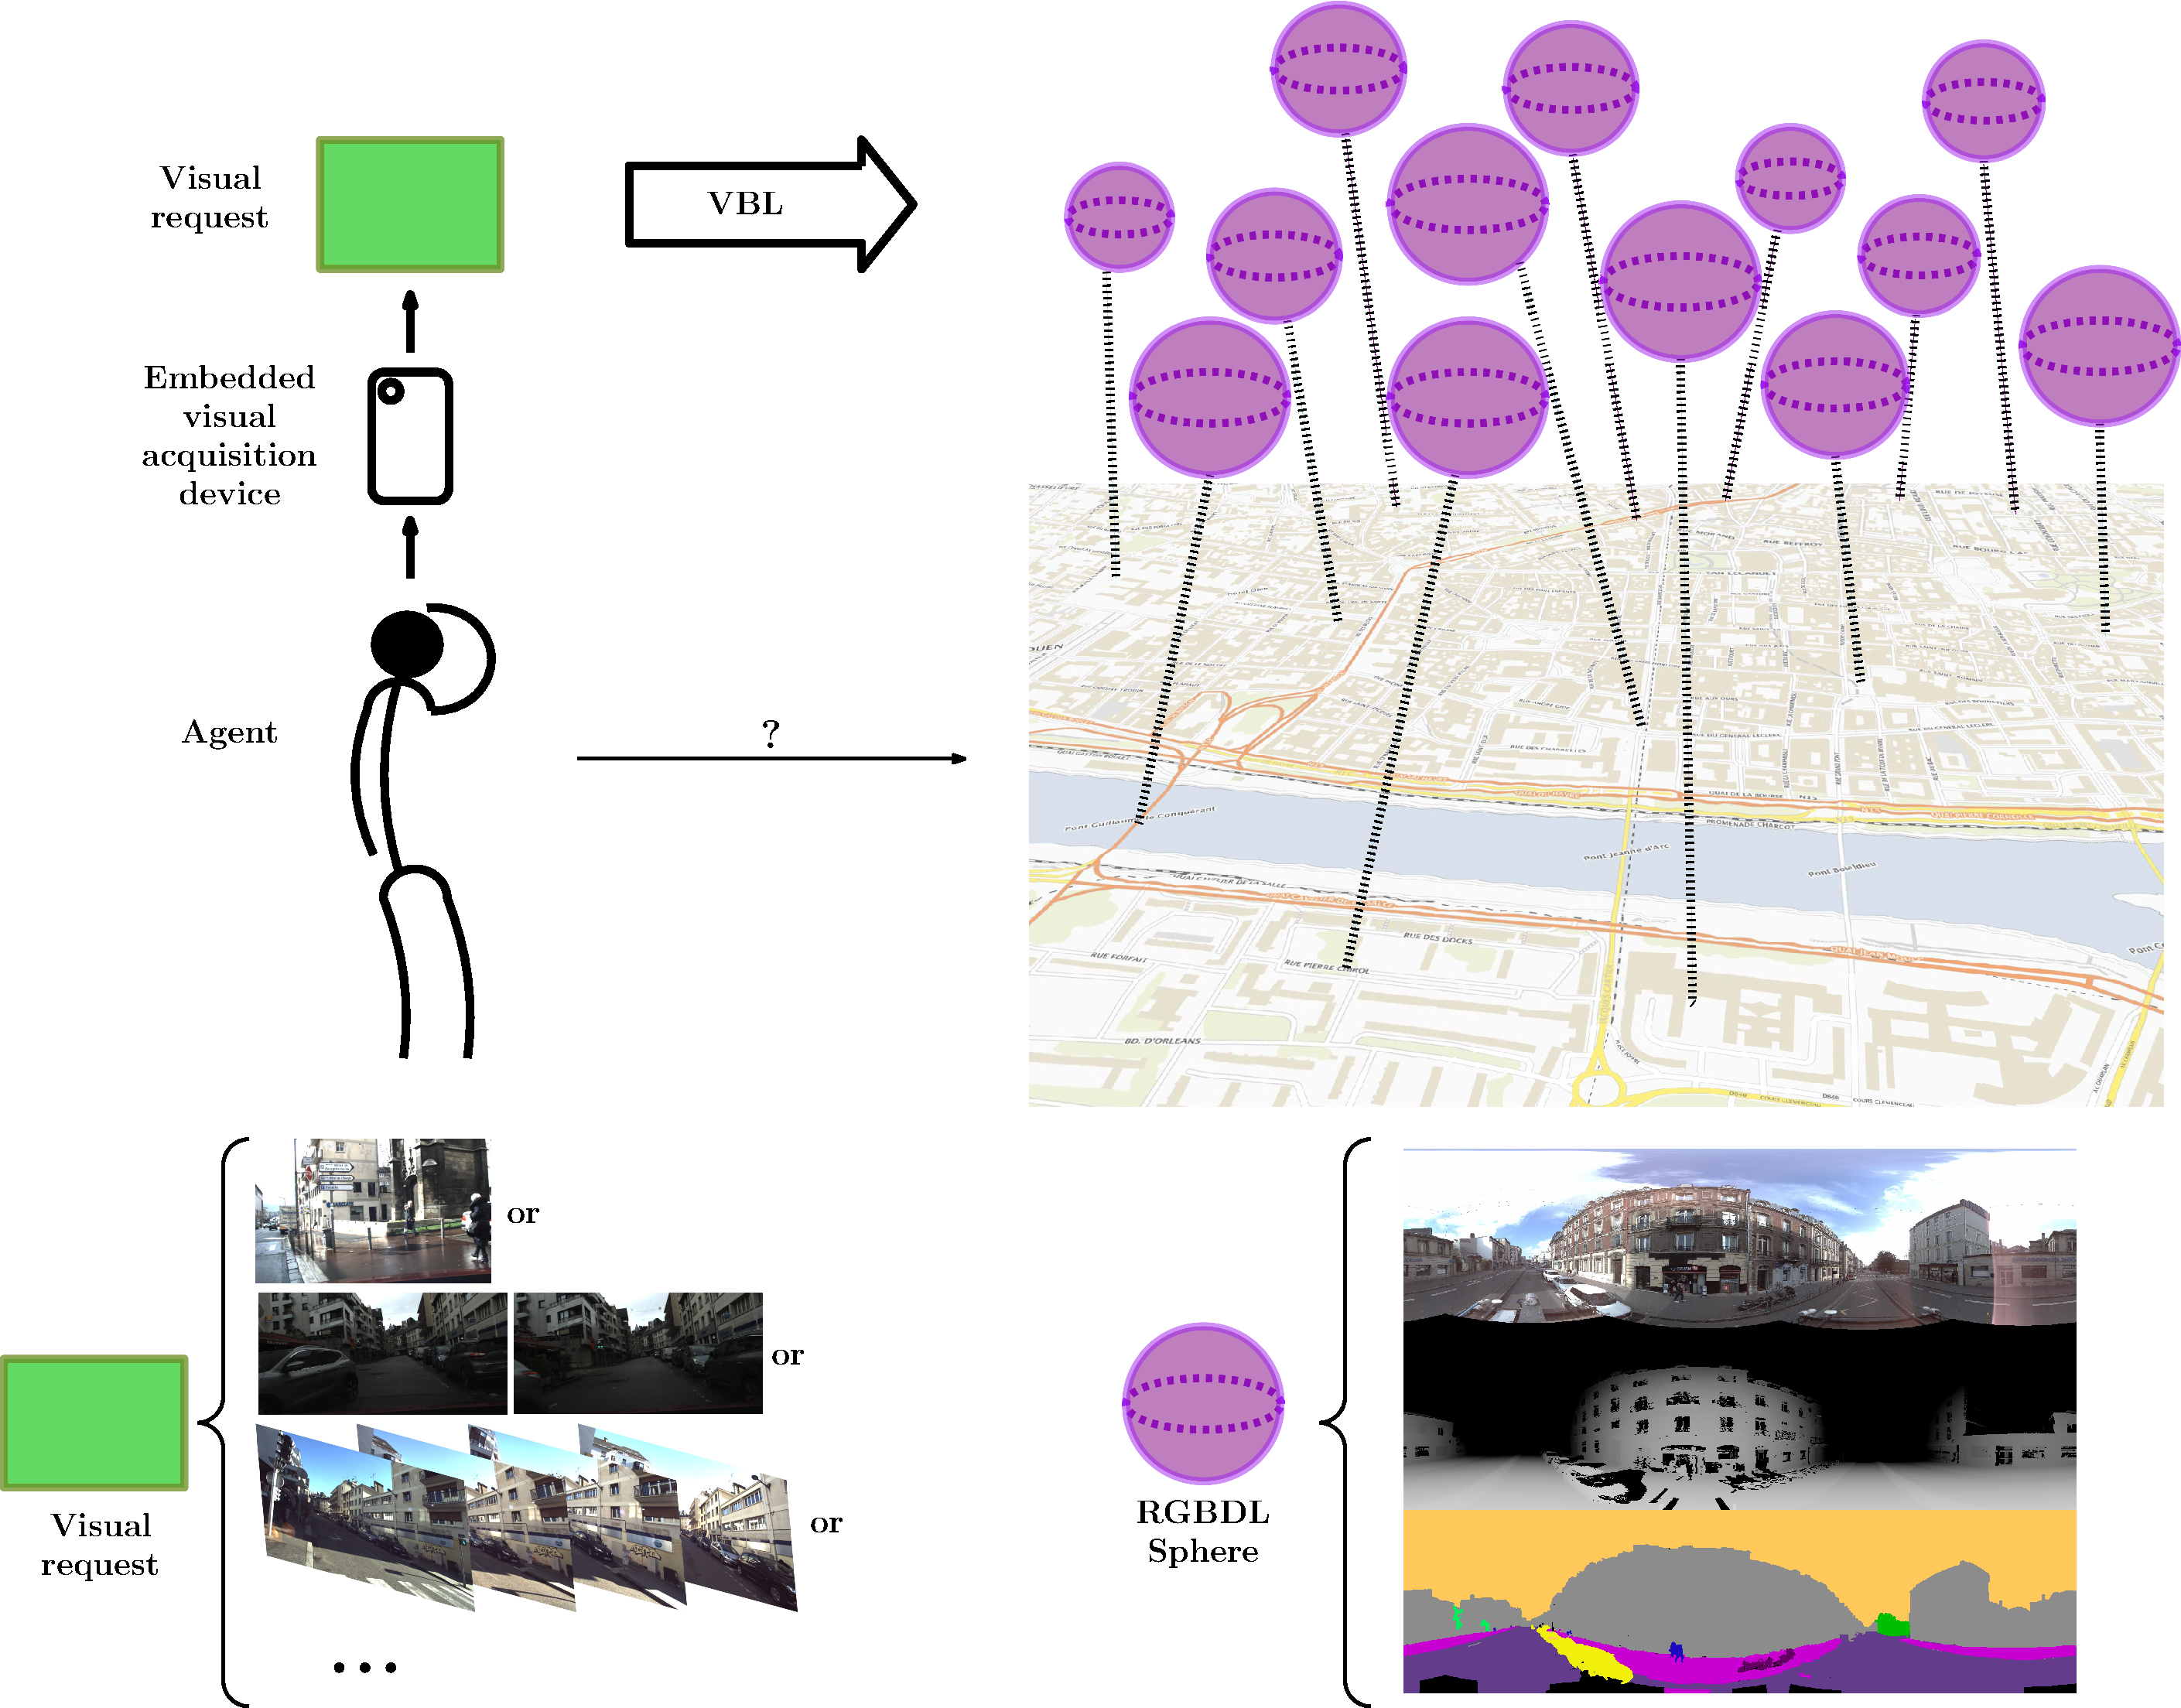
\includegraphics[width=\linewidth]{env/plat_resume}
	\caption[Localization task in \acs*{plat}]{\textbf{The localization task within the \acs*{plat} project:} \label{fig:plat_pipeline} }
\end{figure}


We present in figure~\ref{fig:plat_pipeline} the localization task considered within the \ac{plat} project.